\section{Harun Ar - Rasyid}
\subsection{Penangganan error}
dalam praktek kali ini alhamdulliha tidak menemukan error

%%%%%%%%%%%%%%%%%%%%%%%%%%%%%%%%%%%%%%%%%%%%%%%%%%%%%%%%%%%%%

\section{Kadek Diva Krishna Murti}
\begin{enumerate}
	\item Tuliskan  peringatan  error  yang  didapat  dari  mengerjakan  praktek  keempat  ini, dan  jelaskan  cara  penanganan  error  tersebut.   dan  Buatlah  satu  fungsi  yang menggunakan gunakan try except untuk menanggulangi error tersebut.
	
	Peringatan error di praktek keempat ini, yaitu:
	\begin{itemize}
		\item Syntax Errors
		Syntax Errors adalah suatu keadaan saat kode python mengalami kesalahan penulisan. Solusinya adalah memperbaiki penulisan kode yang salah.
		
		\item Name Error
		NameError adalah exception yang terjadi saat kode melakukan eksekusi terhadap local name atau global name yang tidak terdefinisi. Solusinya adalah memastikan variabel atau function yang dipanggil ada atau tidak salah ketik.
		
		\item Type Error
		TypeError adalah exception yang akan terjadi apabila pada saat dilakukannya eksekusi terhadap suatu operasi atau fungsi dengan type object yang tidak sesuai. Solusi dari error ini adalah mengkoversi varibelnya sesuai dengan tipe data yang akan digunakan.
	\end{itemize}
	
	Fungsi yang menggunakan try except
	\lstinputlisting[caption= Fungsi yang menggunakan try except .,firstline=55, lastline=67]{src/1174006/Chapter4/1174006.py}
\end{enumerate}

\textbf{Kode Program}
\begin{figure}[H]
	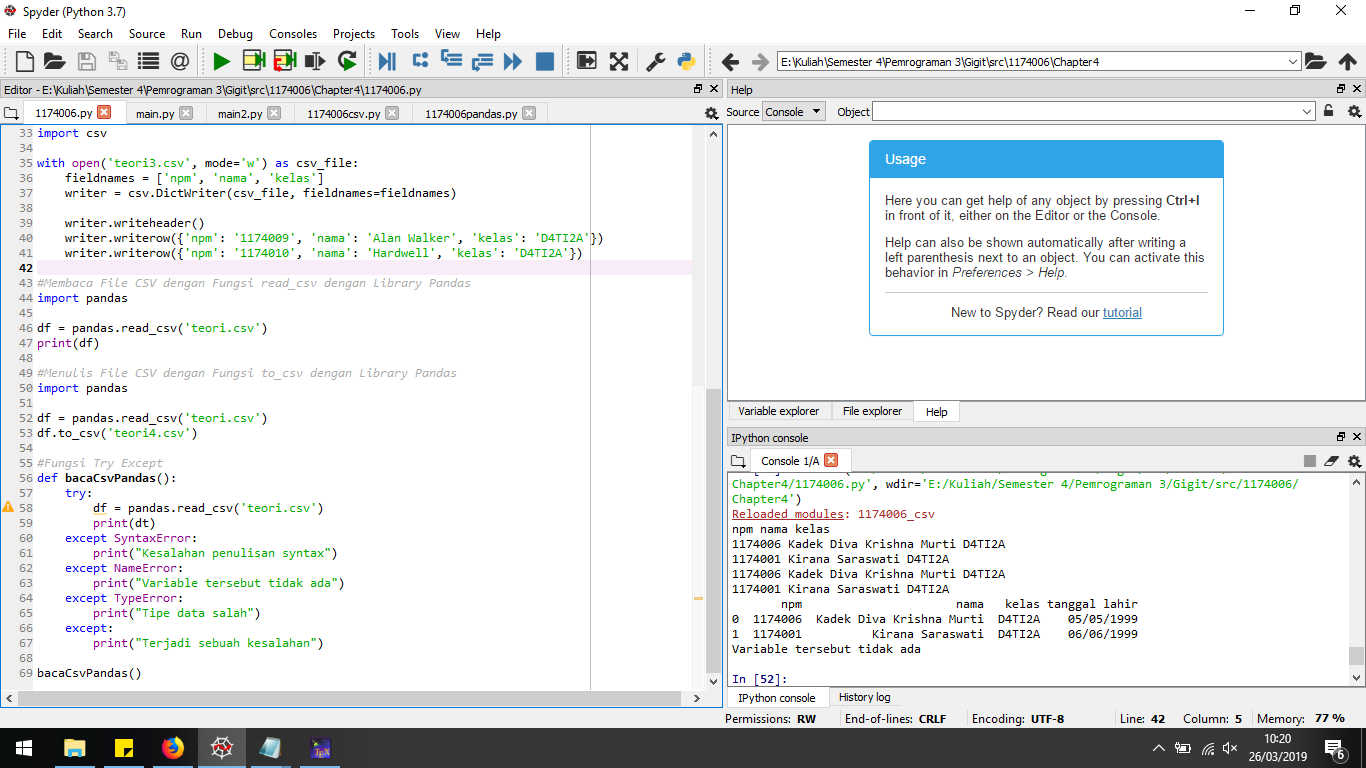
\includegraphics[width=10cm]{figures/diva/Chapter4/harikedua/p1.png}
	\centering
\end{figure}

\textbf{Cek Plagiat}
\begin{figure}[H]
	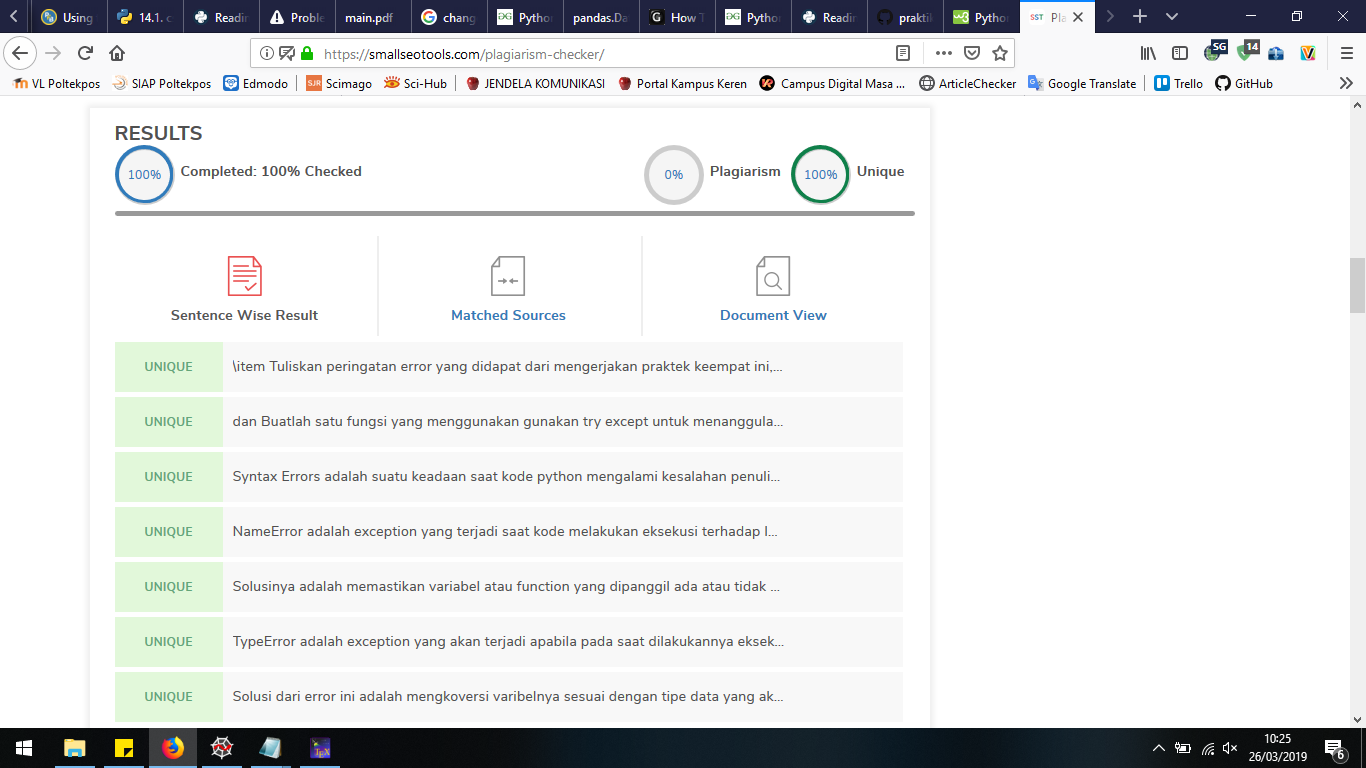
\includegraphics[width=10cm]{figures/diva/Chapter4/harikedua/plagiatpenanganan.png}
	\centering
\end{figure}

%%%%%%%%%%%%%%%%%%%%%%%%%%%%%%%%%%%%%%%%%%%%%%%%%%%%%%%%%%%%%%%%%%%%%%%%%%%%%%%%%%%%%%